\documentclass{article}
\usepackage[utf8]{inputenc}
\usepackage{graphicx}
\usepackage{wrapfig}
\usepackage[T1]{fontenc}
\usepackage{amssymb}
\usepackage{siunitx}

\title{Speed Control of a DC motor by Armature Voltage Control}
\author{Aditya Agrawal\\2021AM10198\\GROUP 29}
\date{June 22,2022}

\begin{document}
\maketitle
\tableofcontents
\newcolumntype{V}{>{\centering\arraybackslash} m{.4\linewidth} }
\newpage

\section{Aim}
Control the speed of the motor using armature voltage control method. Demonstrate motor running at, (i) the rated speed, (ii) half the rated speed.

\section{Apparatus Required}
\begin{enumerate}
    \item 555 Timer and variable resistance
    \item Capacitors and diodes
    \item DSO,wires and power supply
    \item BJT Transistor
    \item DC Motor
\end{enumerate}

\section{Theory}
\begin{wrapfigure}{R}{0.2\textwidth}
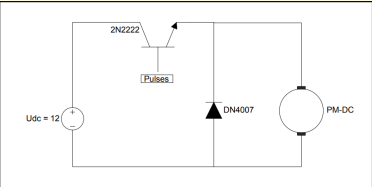
\includegraphics[width=0.5\textwidth]{pic1.png}
\end{wrapfigure}
PWM (Pulse Width Modulation) is a method
through which we can generate variable voltage
by turning on and off the power that’s going to
the electronic device at a fast rate. The average
voltage depends on the duty cycle of the signal,
or the amount of time the signal is ON versus
the amount of time the signal is OFF in a single
period of time.\par
The 555 Timer is capable of generating PWM signal when set up in an astable mode. When the output is HIGH when the capacitor $C_1$ is charging through the resistors $R_1$ and $R_2$. On the other hand, the output of the IC is LOW when the capacitor $C_1$ is discharging but only through the resistor $R_2$. So we can notice that if we change the values of any of these three components we will get different ON and OFF times, or different duty cycle of the square wave output signal. The control pin of the 555 Timer is not used but it’s connected to a 10nF capacitor in order to eliminate any external noise from that terminal.
The reset, pin number 4, is active low so therefore it is connected to VCC in order to prevent any unwanted reset of the output. The output of the 555 timer can sink or source a current of 200mA to the load. So if the motor that we want to control exceeds this rating we need to use a transistor or a MOSFET for driving the motor. We used a (TIP122) Darlington transistor which can handle a current up to 5A. For preventing any voltage spikes produced by the motor we need to use a freewheeling diode which is connected in parallel with the motor.
\newpage

\section{Circuit Diagram}
\begin{figure}[h!]
    \centering
    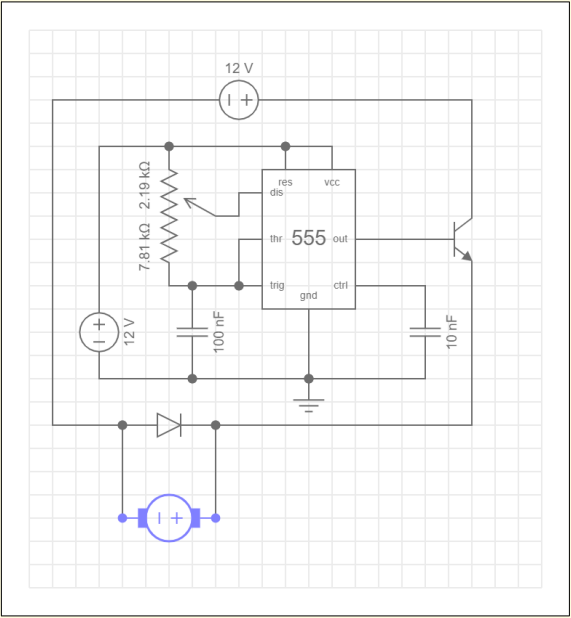
\includegraphics[width=0.9\textwidth]{pic2.png}
    \caption{Circuit Diagram}
\end{figure}
\newpage
\section{Breadboard Setup}
\begin{figure}[h!]
    \centering
    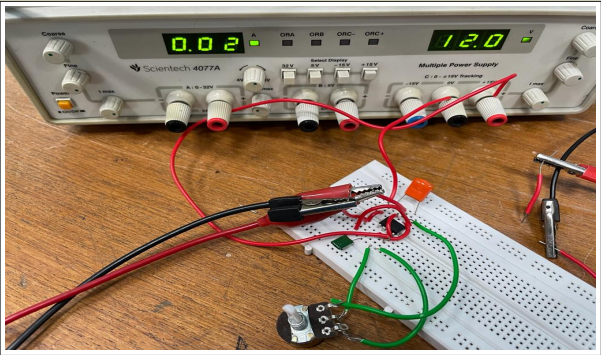
\includegraphics[width=1\textwidth]{pic3.png}
    \caption{Control Circuit}
\end{figure}

\begin{figure}[h!]
    \centering
    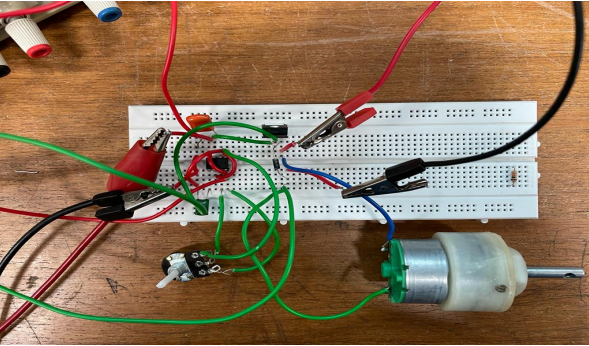
\includegraphics[width=1\textwidth]{pic4.png}
    \caption{Power Circuit}
\end{figure}

\section{DSO Images}
\subsection{Control Circuit}
\begin{center}
    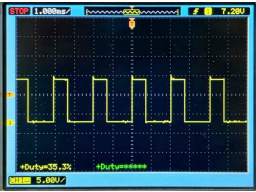
\includegraphics[width=0.4\textwidth]{pic5.png} \hspace{2mm}
    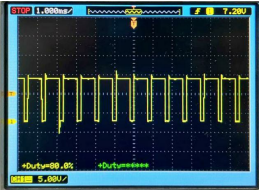
\includegraphics[width=0.4\textwidth]{pic6.png}\\
\end{center}
\subsection{Power Circuit}
\begin{center}
    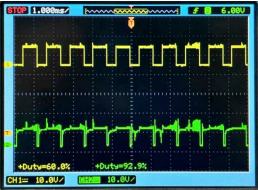
\includegraphics[width=0.4\textwidth]{pic7.png}\hspace{2mm}
    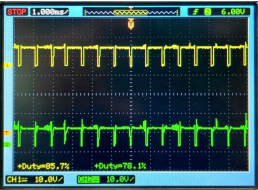
\includegraphics[width=0.4\textwidth]{pic8.png}\\
\end{center}

\section{Sources Of Error}
\begin{itemize}
    \item Scale of DSO not appropriate for measurements.
    \item Resistance of wires not taken into account, and also giving rise to inconsistency due to increase in resistance due to heating.
    \item Loose Connections.
    \item Change in the connections while circuit is closed.
\end{itemize}

\section{Precautions}
\begin{itemize}
    \item Make the connections neat and tight.
    \item Wear proper shoes and use insulated tools.
    \item Don’t leave the switch on for long continuous periods of time.
\end{itemize}
\section{Concluding Remarks}
On the DSO, the output waveform for different values of $R_{1}$ and $R_2$ can be examined by connecting a potentiometer. We notice the following:
\begin{enumerate}
\item The value of $R_1$ should not tend to 0 $\Omega$. The circuit malfunctions if the value is close to 0 $\Omega$. Thus, in ideal case, we should keep $R_{1}$ constant and vary $R_2$. Value of $R_1$ should be kept as low as 1k$\Omega$ while $R_2$ should have a potentiometer of value 100k$\Omega$.
\item We verified that the waveform across the motor and output terminal of IC 555 Timer is same.
\item When we decrease $R_2$, the speed of motor increases and when $R_2$ is 0 $\Omega$, then motor runs at maximum speed.
\item The Darlington transistor (TIP122) is a NPN Transistor. It acts as a switch in our case. When the output waveform is 0V, the transistor is in OFF State.
\item A Freewheeling Diode is connected across the motor. When the Transistor
is in OFF State, it helps the inductive load to freewheel the energy.
\end{enumerate}
\section{Team Members}
\begin{enumerate}
    \item Aditya Agrawal - 2021AM10198
    \item Yash Agarwal - 2021EE10638
    \item Yogesh Yadav - 2021CH10406
\end{enumerate}

\end{document}
